\subsubsection{ACI Visualization}
As ACI is best represented over a period of time, the first infographic that comes to mind for representing it is a line chart. Naturally, a line chart can represent date and time in the X axis and the ACI value in the Y axis. Additionally, a bar chart for showing the overall ACI value for a data set as a whole would be useful. Researchers organize their data in different ways, and it is important to provide as many different graphs as possible to try to accommodate the research goal. The ACI index has the most graphs available because of this.\par

\begin{center}
  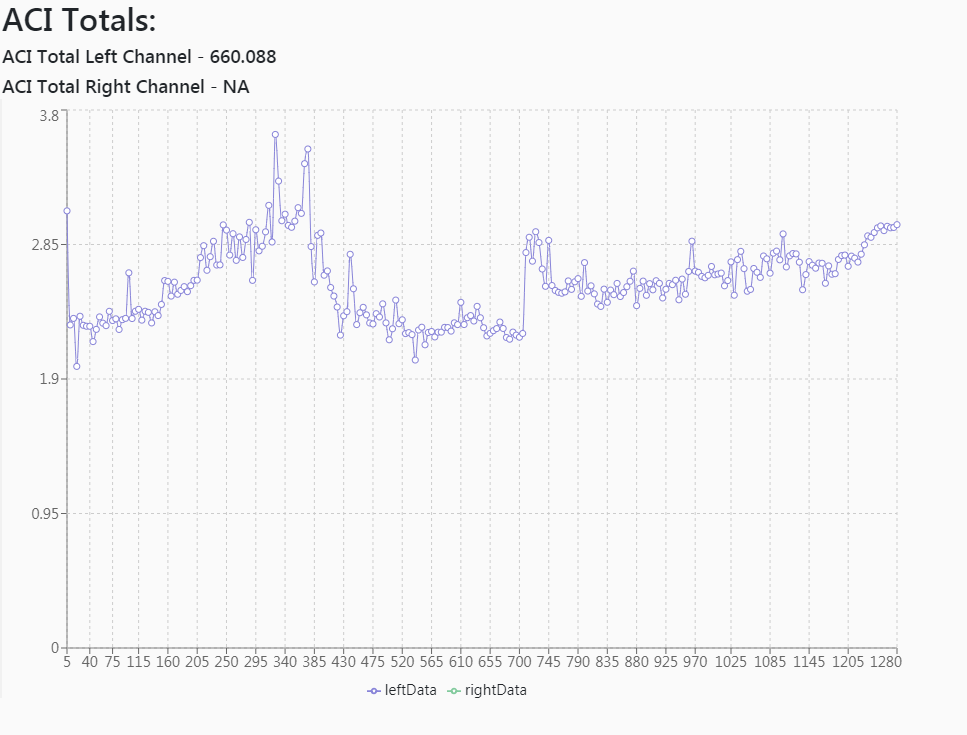
\includegraphics[width=\textwidth]{ACIgraph1} \\[12pt]
\end{center}
The first graph available shows all the files in the set, in order in which they appear in the set. Further, each data point represents a time stamp in that file. The X axis here represents the name of the file, and if you hover over a data point, it will detail at what time stamp in the file did that data occur. Here, an audio player is also available if you click on any data point, and it will even begin playback at that time stamp.\par

\begin{center}
  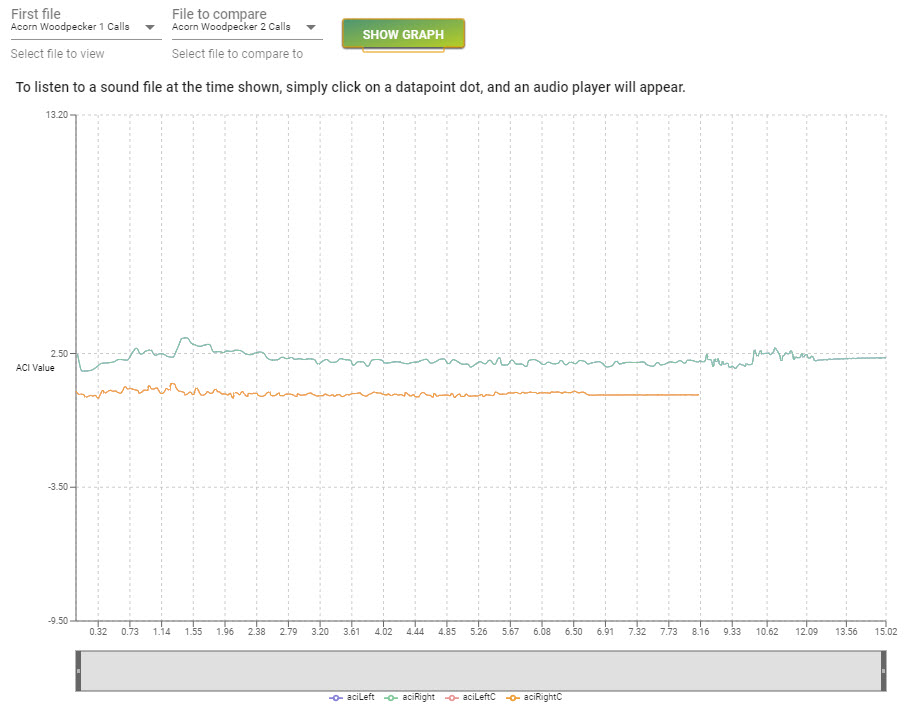
\includegraphics[width=\textwidth]{ACIgraph2} \\[12pt]
\end{center}
This graph aims to compare individual files in a data set much like the first graph. Here, you can examine a single file or compare two files in the chosen Site and/or Series. Again, an audio player is available and can also begin playback at the designated time stamp.\par

\begin{center}
  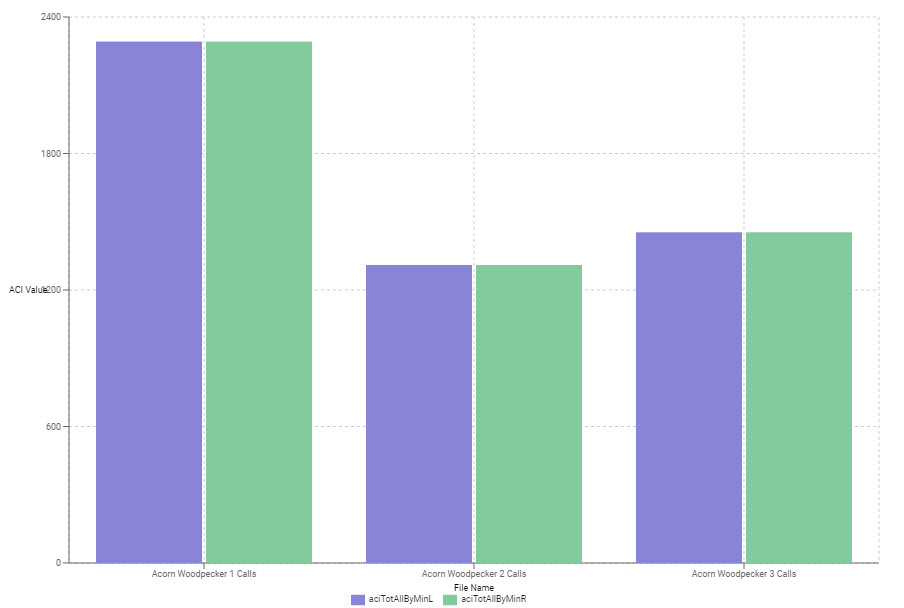
\includegraphics[width=\textwidth]{ACIgraph3} \\[12pt]
\end{center}
This graph differs from the first two as it is a bar chart and it also represents overall ACI value for the file rather than over time of the file. Here, each file gets its own Bar representation with each channel. This graph is useful to see overall ACI value as it changes from file to file.\par

\begin{center}
  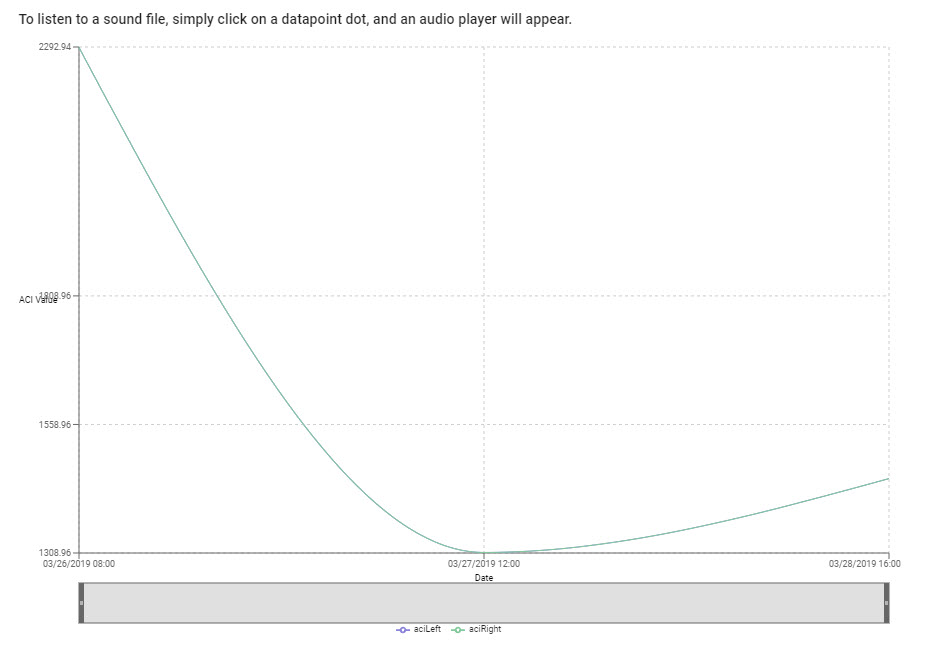
\includegraphics[width=\textwidth]{ACIgraph4} \\[12pt]
\end{center}
The last two graphs available for ACI are for showing ACI by date and time and by file. These are simple line graphs that include the ACI value at the given date and time or by the given file.
